\documentclass{article}

\usepackage{graphicx}
\usepackage{tikz}
\usepackage{tikzsymbols}
\usetikzlibrary{calc,patterns,shapes.geometric}
\pagestyle{empty}
\usepackage[margin=0pt]{geometry}
\geometry{papersize={14in,12in}}

\def\centerarc[#1](#2)(#3:#4:#5){\draw[#1] ($(#2)+({#5*cos(#3)},{#5*sin(#3)})$) arc (#3:#4:#5);}

\begin{document}
	\begin{figure}
		\centering
		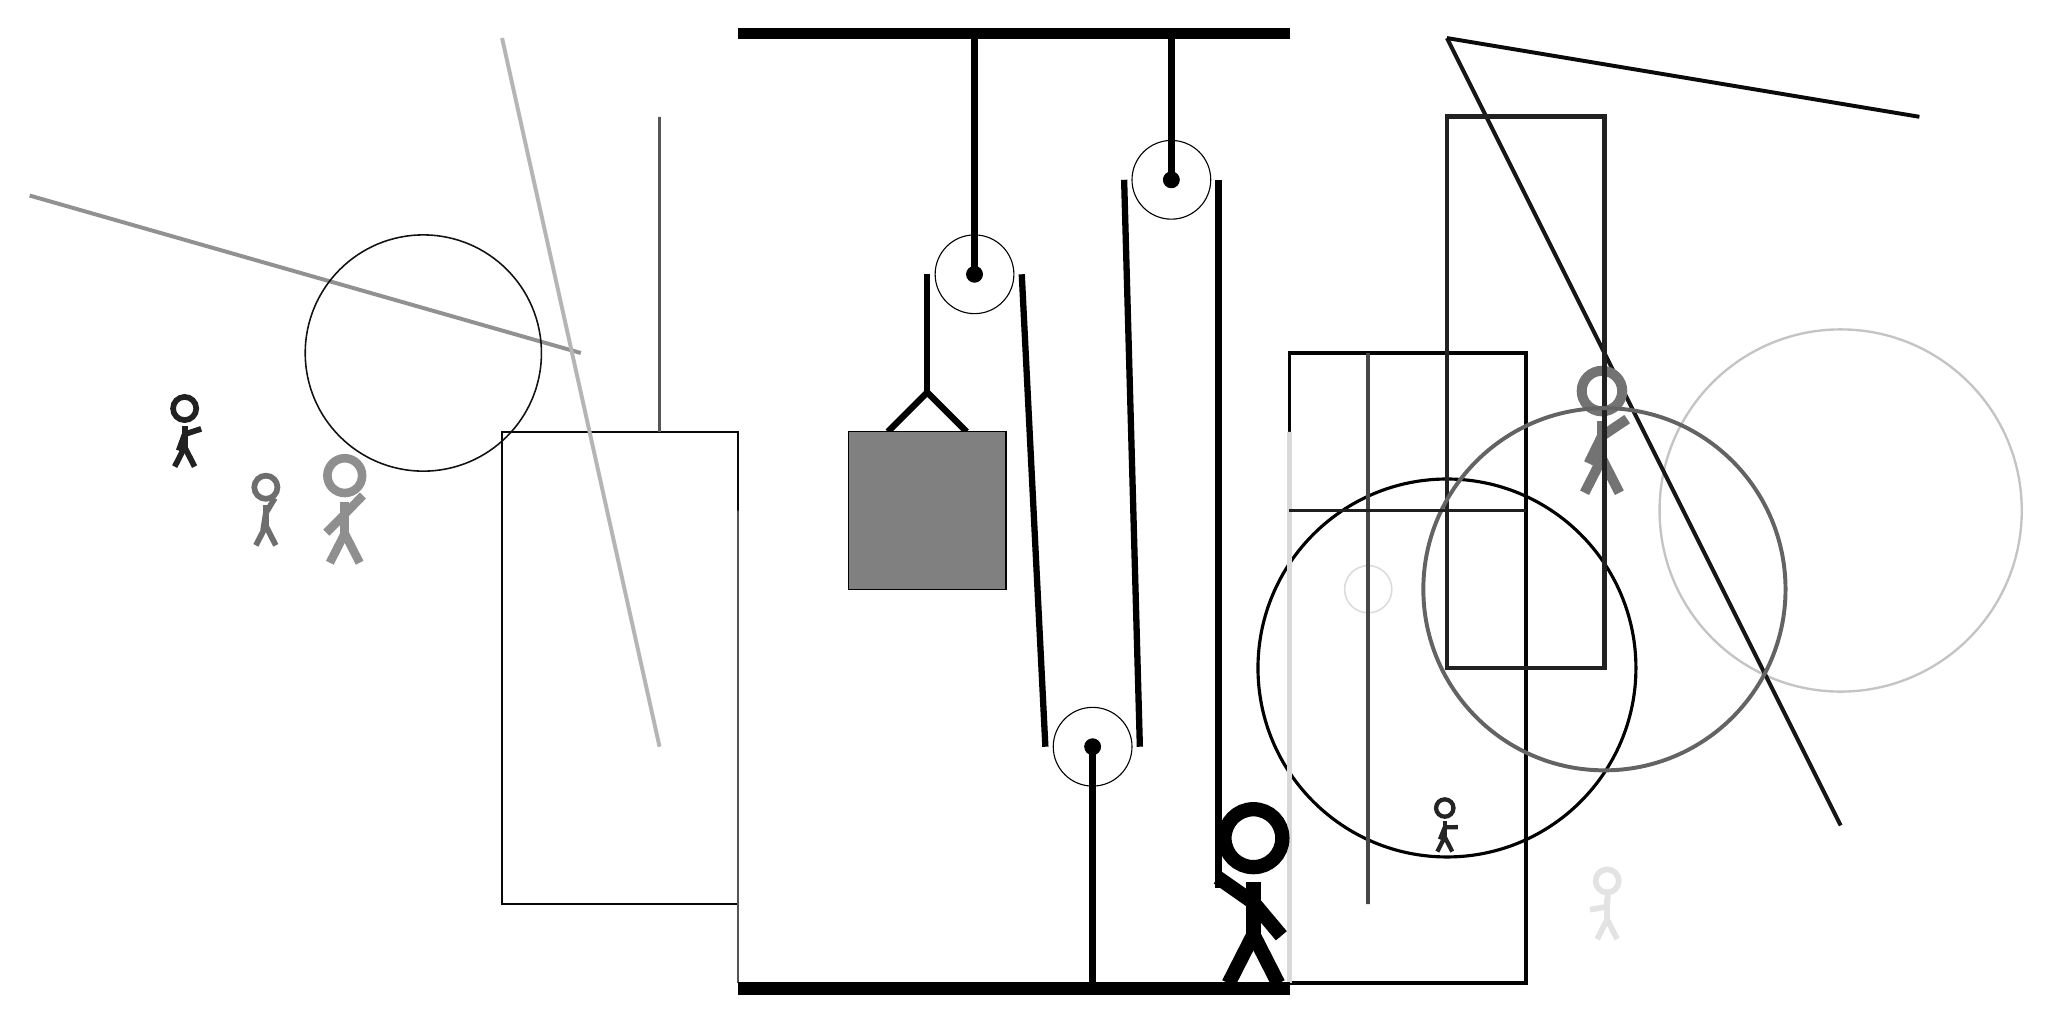
\begin{tikzpicture}
			%%%%% START %%%%%
			
			\draw[fill=black] (-2, 9) rectangle (5, 9.125);
			
			\draw (1, 6) circle (0.5);
			\draw[fill=black] (1, 6) circle (0.1);
			\draw[line width=0.8mm]  (1, 9) -- (1, 6);
			
			\draw[line width=0.3mm, color=black!97] (-2, 4) rectangle (-5, -2);
			
			\draw[line width=0.5mm, color=black!43](-4, 5) -- (-11, 7);
			\node[line width=0.6mm, color=black!86] at (7, -1) {\Strichmaxerl[3][68][1]};
			\draw[line width=0.5mm, color=black!29](-3, 0) -- (-5, 9);
			
			\draw [line width=0.4mm, color=black!100](7, 1) circle (2.4);
			\node[line width=0.5mm, color=black!44] at (-7, 3) {\Strichmaxerl[6][45][46]};
			\draw[line width=0.3mm, color=black!67] (-2, 3) rectangle (-2, -3);
			\draw[line width=0.5mm, color=black!99] (5, -3) rectangle (8, 5);
			\draw [line width=0.3mm, color=black!23](12, 3) circle (2.3);
			
			\draw [line width=0.2mm, color=black!14](6, 2) circle (0.3);
			
			\draw[line width=0.5mm, color=black!91](7, 9) -- (12, -1);
			
			\node[line width=0.3mm, color=black!55] at (9, 4) {\Strichmaxerl[7][64][34]};
			\draw[line width=0.5mm, color=black!96](7, 9) -- (13, 8);
			
			\draw [line width=0.2mm, color=black!93](-6, 5) circle (1.5);
			\draw [line width=0.7mm, color=black!87](7, 8) circle (0.0);
			\node[line width=0.2mm, color=black!11] at (9, -2) {\Strichmaxerl[4][10][87]};
			\draw[line width=0.5mm, color=black!72] (6, -2) rectangle (6, 5);
			
			\draw[line width=0.6mm, color=black!87] (7, 1) rectangle (9, 8);
			\draw [line width=0.5mm, color=black!61](9, 2) circle (2.3);
			\draw[line width=0.6mm, color=black!15] (5, -3) rectangle (5, 4);
			\draw[line width=0.5mm, color=black!88](5, 3) -- (8, 3);
			\draw[line width=0.3mm, color=black!66] (-3, 8) rectangle (-3, 4);
			\node[line width=0.3mm, color=black!87] at (-9, 4) {\Strichmaxerl[4][70][18]};
			\node[line width=0.3mm, color=black!57] at (-8, 3) {\Strichmaxerl[4][81][59]};
			
			\draw[fill=white](2.5, 0) circle (0.5);
			\draw[fill=black] (2.5, 0) circle (0.1);
			\draw[line width=0.8mm]  (2.5, -3) -- (2.5, 0);
			
			\draw[fill=white](3.5, 7.2) circle (0.5);
			\draw[fill=black] (3.5, 7.2) circle (0.1);
			\draw[line width=0.8mm] (3.5, 9) -- (3.5, 7.2);
			
			\draw[line width=0.8mm] (-0.1, 4.0) -- (0.4, 4.5) -- (0.9, 4.0);
			\draw[fill=black!50] (-0.6, 4.0) rectangle (1.4, 2.0);
			
			\draw[line width=0.8mm] (0.4, 6) -- (0.4, 4.5);
			\centerarc[line width=0.8mm](1, 6)(0:180:0.6);
			\draw[line width=0.8mm](1.6, 6) -- (1.9, 0);
			\centerarc[line width=0.8mm](2.5, 0)(180:360:0.6);
			\draw[line width=0.8mm](3.1, 0) -- (2.9, 7.2);
			\centerarc[line width=0.8mm](3.5, 7.2)(0:180:0.6);
			\draw[line width=0.8mm](4.1, 7.2) -- (4.1, -1.8);
			
			\node at (4.5, -1.9) {\Strichmaxerl[10][-35][-50]};
			
			\draw[fill=black] (-2, -3) rectangle (5, -3.15);
			
			%%%%% END %%%%%
		\end{tikzpicture}
	\end{figure}	
\end{document}